\documentclass{article}

\usepackage{longtable}


\usepackage{Sweave}
\begin{document}
\Sconcordance{concordance:A_guide_to_GUIDE.tex:A_guide_to_GUIDE.Rnw:%
1 5 1 1 0 21 1 1 2 4 0 1 2 1 1 1 2 4 0 1 2 2 1 1 2 4 0 1 2 157 1}

% \VignetteIndexEntry{A guide to GUIDE}


\author{S Subramanian\\
Dept. of Management Studies\\ Sri Sathya Sai Institute of Higher Learning\\ Prasanthi Nilayam, A.P. INDIA. 515134.\\
Email: ssubramanian@sssihl.edu.in\\} 
\title{A guide to GUIDE}


\maketitle

\begin{abstract}{
This paper is a guide to the R package GUIDE, short for GUI for DErivatives.The installation of package is described followed by a listing of the menus and depiction of select screenshots.}
\end{abstract}

\section{Introduction}
GUIDE is an acronym for for GUI for DErivatives. The package provides neat UIs like calculators for pricing various financial derivatives as well as rich interactive 2D and 3D plots to understand their behavior. It is a useful resource for classroom teaching as well as computer assisted self-learning. 

\section{Installation}
 Installation is easy and can be done by calling the command line function
\begin{Schunk}
\begin{Sinput}
> install.packages("GUIDE")
\end{Sinput}
\end{Schunk}

Alternatively, one can also install it from the R console package installation menu. To start using the package, enter 
\begin{Schunk}
\begin{Sinput}
> library("GUIDE")
\end{Sinput}
\end{Schunk}
You can also load the package from the console menu.

To start using the package, enter 
\begin{Schunk}
\begin{Sinput}
> GUIDE()
\end{Sinput}
\end{Schunk}

You should then see the main menu of the package as in Figure \ref{Fig:mainmenu}. 

\section{Menus}
GUIDE has 64 functions. A complete list of functions (in menu-wise order) along with a short description is provided in Table \ref{Tab:fns}


\begin{center}
\begin{longtable}{  l  l  }
\caption{List of Functions in GUIDE}
\\\hline
Name of Function & Description  \\
\hline
\endfirsthead
\multicolumn{2}{c}%
{\tablename\ \thetable\ -- \textit{Continued from previous page}} \\
\hline
Name of Function & Description  \\
\hline
\endhead
\hline \multicolumn{2}{r}{\textit{Continued on next page}} \\
\endfoot
\hline\\
%\caption{List of Functions in GUIDE}
\endlastfoot
\multicolumn{2}{ c }{Forwards} \\                   
forwardcommodity & Calculate the forward value of a commodity \\
forwardcurrency & Calculate the forward value of a currency\\
forwardstock & Calculate the forward value of a stock\\
bondforwardtreegui & Calculate the forward value of a bond using a tree\\
fra & Calculate the forward rate\\
fravalue & Calculate the value of a forward rate agreement\\
\\
\multicolumn{2}{ c }{Futures} \\      
futurescommodity & Calculate the value of a commodity futures\\
futurescurrency & Calculate the value of a currency futures\\
futuresstock & Calculate the value of a stock futures\\
bondfuturestreegui & Calculate the futures value of a bond using a tree\\
eurodollar & Calculate the value of a eurodollar futures contract\\
cashprice & Calculate the Cash price of a T Bond Futures\\
\\
\multicolumn{2}{ c }{Options} \\
basicpayoffs & Plot payoffs / profit and loss of European Call/Put\\
Premium3D & Plot Option premium as a function of stock price/strike and time\\
stockoptiontreegui & Plot a Stock Option Tree\\
bondoptiontreegui & Plot a Bond Option Tree\\
blackscholes & Calculate the Black scholes formula value of a European Call/Put\\
impvol & Calculate the Black scholes implied volatility of a European Call/Put\\
calcgreeks & Calculate the greeks for a European Call/Put\\
stockTimeGreeks & Plot of option greeks as a function of stock price and time\\
greekneutrality & Calculate the hedge positions for  European Call/Put\\
captreegui & Plot a Cap tree\\
floortreegui & Plot a Floor tree\\
bullspreadcalls & Profit \& Loss plot of bull spread with calls\\
bearspreadputs & Profit \& Loss plot of bear spread with puts\\
butterfly & Profit \& Loss plot of butterfly\\
reversebutterfly & Profit \& Loss plot of reverse butterfly\\
straddle & Profit \& Loss plot of straddle\\
reversestraddle & Profit \& Loss plot of reverse straddle\\
strangle & Profit \& Loss plot of strangle\\
reversestrangle & Profit \& Loss plot of reverse strangle\\
strip & Profit \& Loss plot of strip\\
strap & Profit \& Loss plot of strap\\
\\
\multicolumn{2}{ c }{Swaps} \\
irswapvalue & Calculate the value of an interest rate swap\\
curswapvalue & Calculate the value of a fixed-fixed currency swap\\
cdswap & Calculate the spread in a credit default swap\\
swaptreegui & Plot an interest rate swap tree\\
swaptiontreegui & Plot an interest rate swaption tree\\
\\
\multicolumn{2}{ c }{Stochastic Processes} \\
ABMPaths & Simulate and plot Arithmetic Brownian Motion path(s)\\
GBMPaths & Simulate and plot Geometric Brownian Motion path(s)\\
JDPaths & Simulate and plot Jump Diffusion path(s)\\
\\
\multicolumn{2}{ c }{Value at Risk} \\
var1stock & Calculate the value at risk of a single stock\\
var2stocks & Calculate the value at risk of two stocks\\
varbehavior & Plot the value at risk as a function of its determinants\\
\\
\multicolumn{2}{ c }{Bonds} \\
ratetreegui & Plot a interest rate tree\\
bondtreegui & Plot a bond price tree\\
bondprice & Calculate the price of a bond\\
priceyield & Plot the relationship between price and yield of a bond\\
pricematurity & Plot the relationship between price and maturity of a bond\\
bonddur & Calculate the duration of a bond\\
durmaturity & Plot the relationship between duration and maturity of a bond\\
durcoupon & Plot the relationship between duration and coupon rate of a bond\\
duryield & Plot the relationship between duration and yield of a bond\\
bondconv & Calculate the convexity of a bond\\
bondchange & Calculate the DV01 based on the duration and convexity\\
\\
\multicolumn{2}{ c }{Utilities} \\
pv & Calculate the Present value of an amount\\
fv & Calculate the Future value of an amount\\ 
pvann & Calculate the Present value of an annuity\\
fvann & Calculate the Future value of an annuity\\
rate & Calculate rate in the desired frequency\\
pval & Calculate the p value for a z value from a normal distribution\\
zval & Calculate the z value for a p value from a normal distribution\\
%\caption{List of Functions in GUIDE}
\label{Tab:fns}
\end{longtable}
\end{center}


Each of the functions can be accessed from sub menus of the main menu. Sub menu of the Options menu is shown in Figure \ref{Fig:opmenu}. You can fully explore all the functions through the package's GUI and do not need to write any command on the R console. Figures \ref{Fig:calcbs} and \ref{Fig:calcbond} show calculators for the Black Scholes price of Options, and the price of Bonds respectively. Each function depicts initial values where user inputs are needed, thereby making it easier for the user to enter inputs in the correct format. For e.g. in Figure \ref{Fig:calcbs} (b), the Black Scholes pricer takes the following inputs: i) the spot price ii) the strike price iii) the risk free rate iv) maturity, v) sigma, vii) dividend yield- all of which are text boxes and viii)  Type of option, which is a radio button. The documentation provides details of the format for each of the user inputs for each function. Figure \ref{Fig:tkrplotpriceyld} shows the relationship between price and yield. Figure \ref{Fig:nativeplotdelta} shows the behavior of option delta. 

\begin{figure}
\centering
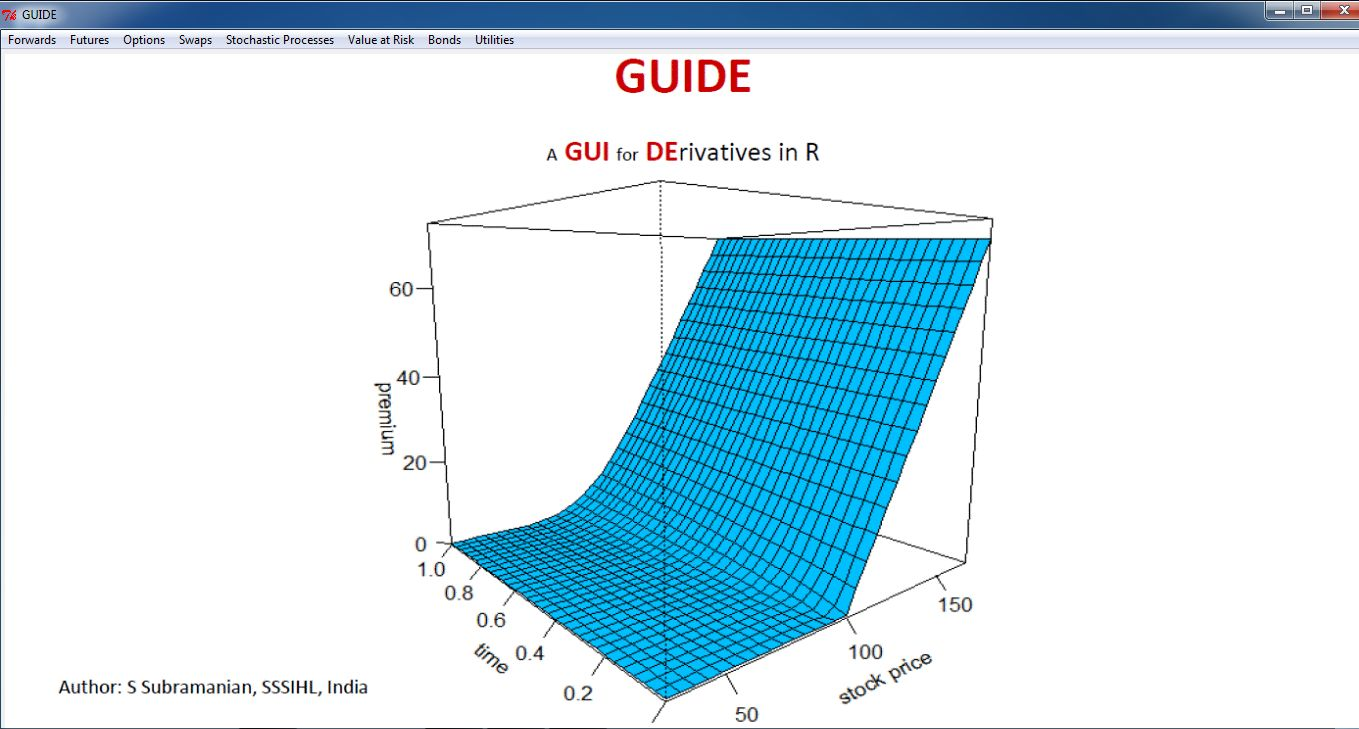
\includegraphics[width=1\textwidth]{guidemain.jpg}
\caption{The Main menu of GUIDE.} 
\label{Fig:mainmenu}
\end{figure}

\begin{figure}
\centering
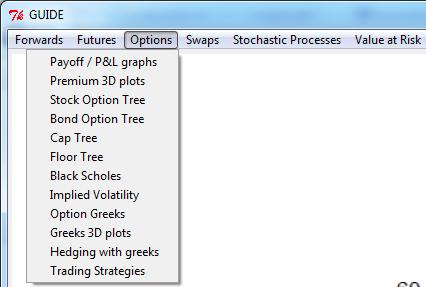
\includegraphics[width=1\textwidth]{op-menu.jpg}
\caption{The sub-menu of Options.} 
\label{Fig:opmenu}
\end{figure}


\begin{figure}
\centering
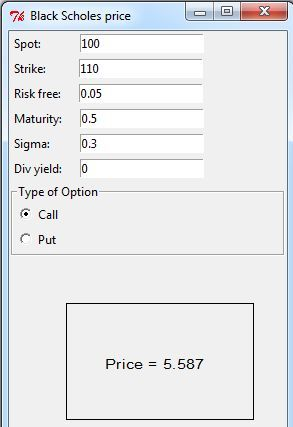
\includegraphics{bs2.jpg}
\caption[]{UI for Black Scholes price.}
\label{Fig:calcbs}
\end{figure}

\begin{figure}
\centering
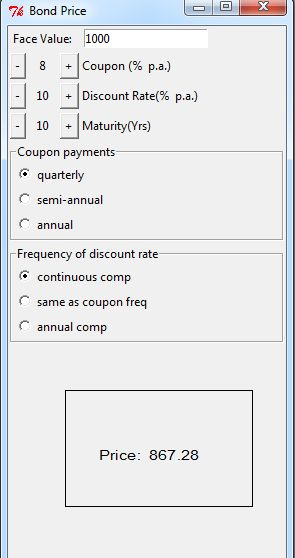
\includegraphics{bondprice.jpg}
\caption[]{UI for bond price.}
\label{Fig:calcbond}
\end{figure}

\begin{figure}
\centering
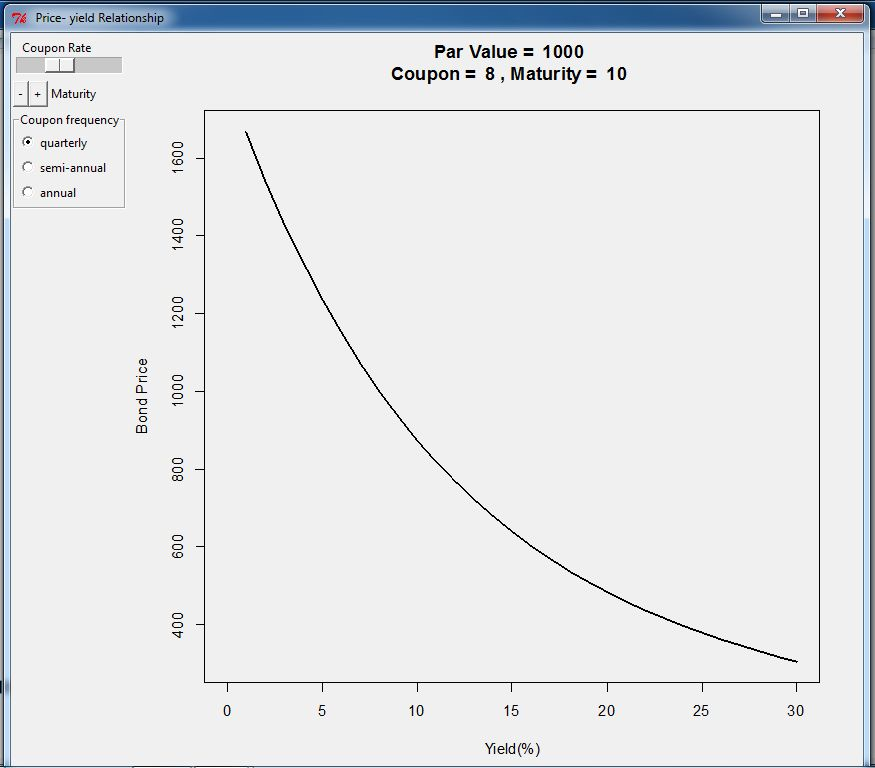
\includegraphics[width=1\textwidth]{priceyield2.jpg}
\caption[]{Price yield relationship plot.}
\label{Fig:tkrplotpriceyld}
\end{figure}

\begin{figure}
\centering
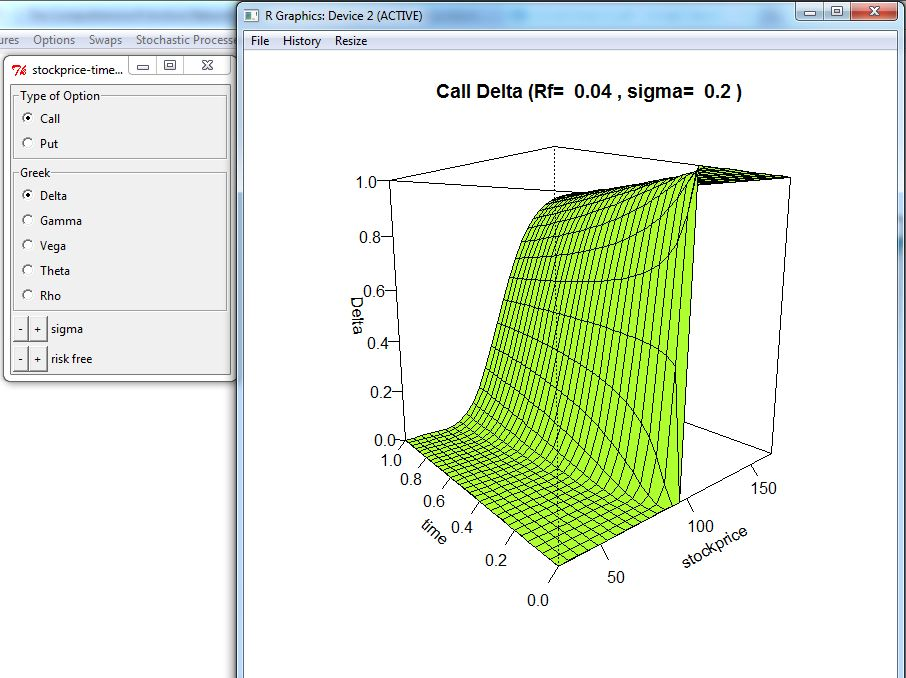
\includegraphics[width=1\textwidth]{delta.jpg}
\caption[]{Behavior of Option delta.}
\label{Fig:nativeplotdelta}
\end{figure}



\end{document}


